% !TeX root = ../main.tex
\section{Результаты имитационного моделирования}

Моделирование тракта цифровой демодуляции и согласованной фильтрации проводилось в среде MATLAB в соответствии с параметрами варианта~8 ($f_c = 210.0$~МГц, $f_s = 180.0$~МГц, $n_a = n_g = 13$~бит). Отношение сигнал/шум на входе тракта составляло $\text{SNR} = 50$~дБ, а все промежуточные расчеты выполнялись в формате с плавающей запятой двойной точности (\texttt{double}).

На первом этапе был сформирован симметричный ЛЧМ-радиоимпульс длительностью $T_{\text{и}} = 25.6$~мкс ($N_{\text{имп}} = 4608$ отсчетов), задержанный на интервал $N_{\text{del}} = 8192$ отсчета относительно начала периода зондирования. После оцифровки, квадратурного гетеродинирования и низкочастотной фильтрации на вход блока согласованной фильтрации поступает комплексный видеосигнал, огибающая которого представлена на рисунке~\ref{fig:in_bb}.

\begin{figure}[H]
    \centering
    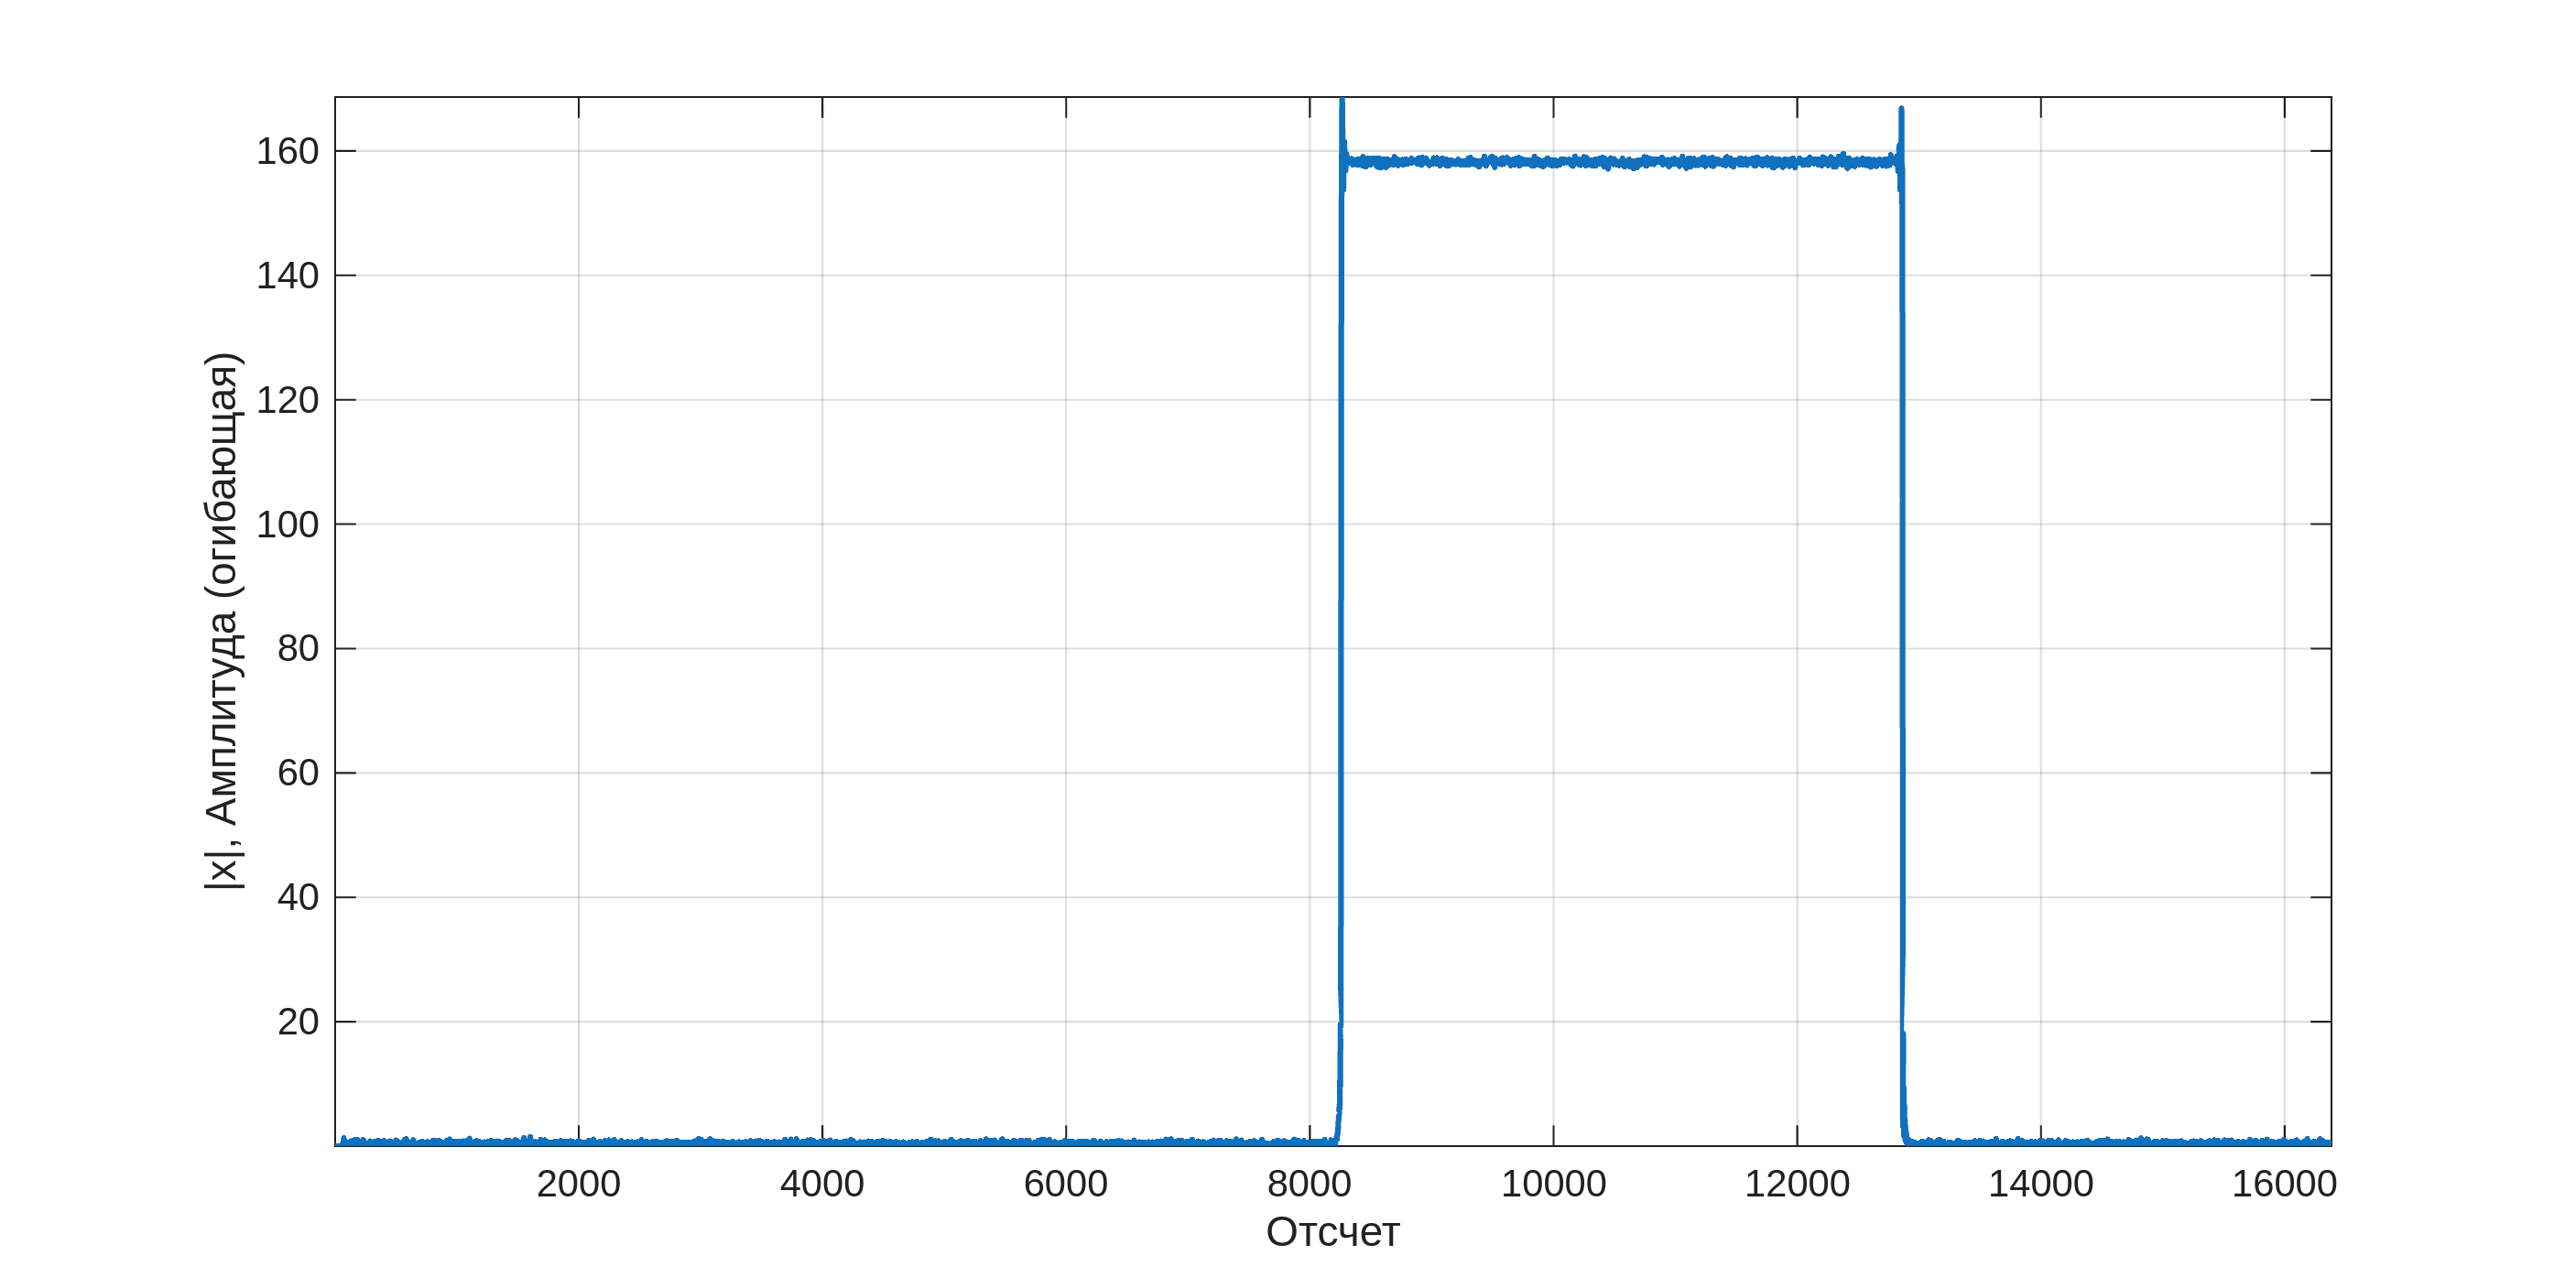
\includegraphics[width=0.85\textwidth]{export_figs/fig_input_bb.png}
    \caption{Огибающая комплексного видеосигнала на входе СФ после ЦДМ и ЦФ}
    \label{fig:in_bb}
\end{figure}

Анализ временной диаграммы показывает, что видеоимпульс сохраняет прямоугольную форму длительностью ровно $4608$ отсчетов (интервал от отсчета $8192$ до $12800$). Высокочастотные продукты преобразования частоты и внеполосные помехи эффективно подавлены фильтром нижних частот 128-го порядка, а спектральных искажений огибающей не наблюдается.

Далее была выполнена согласованная фильтрация тремя алгоритмами без применения весового окна: во временной области прямой сверткой (FIR), в частотной области через БПФ/ОБПФ (FFT/IFFT) и блочным методом сегментированной свертки с накоплением (\texttt{fftfilt}). На рисунке~\ref{fig:mf_compare} приведено совместное наложение нормированных откликов фильтра во всем окне периода зондирования.

\begin{figure}[H]
    \centering
    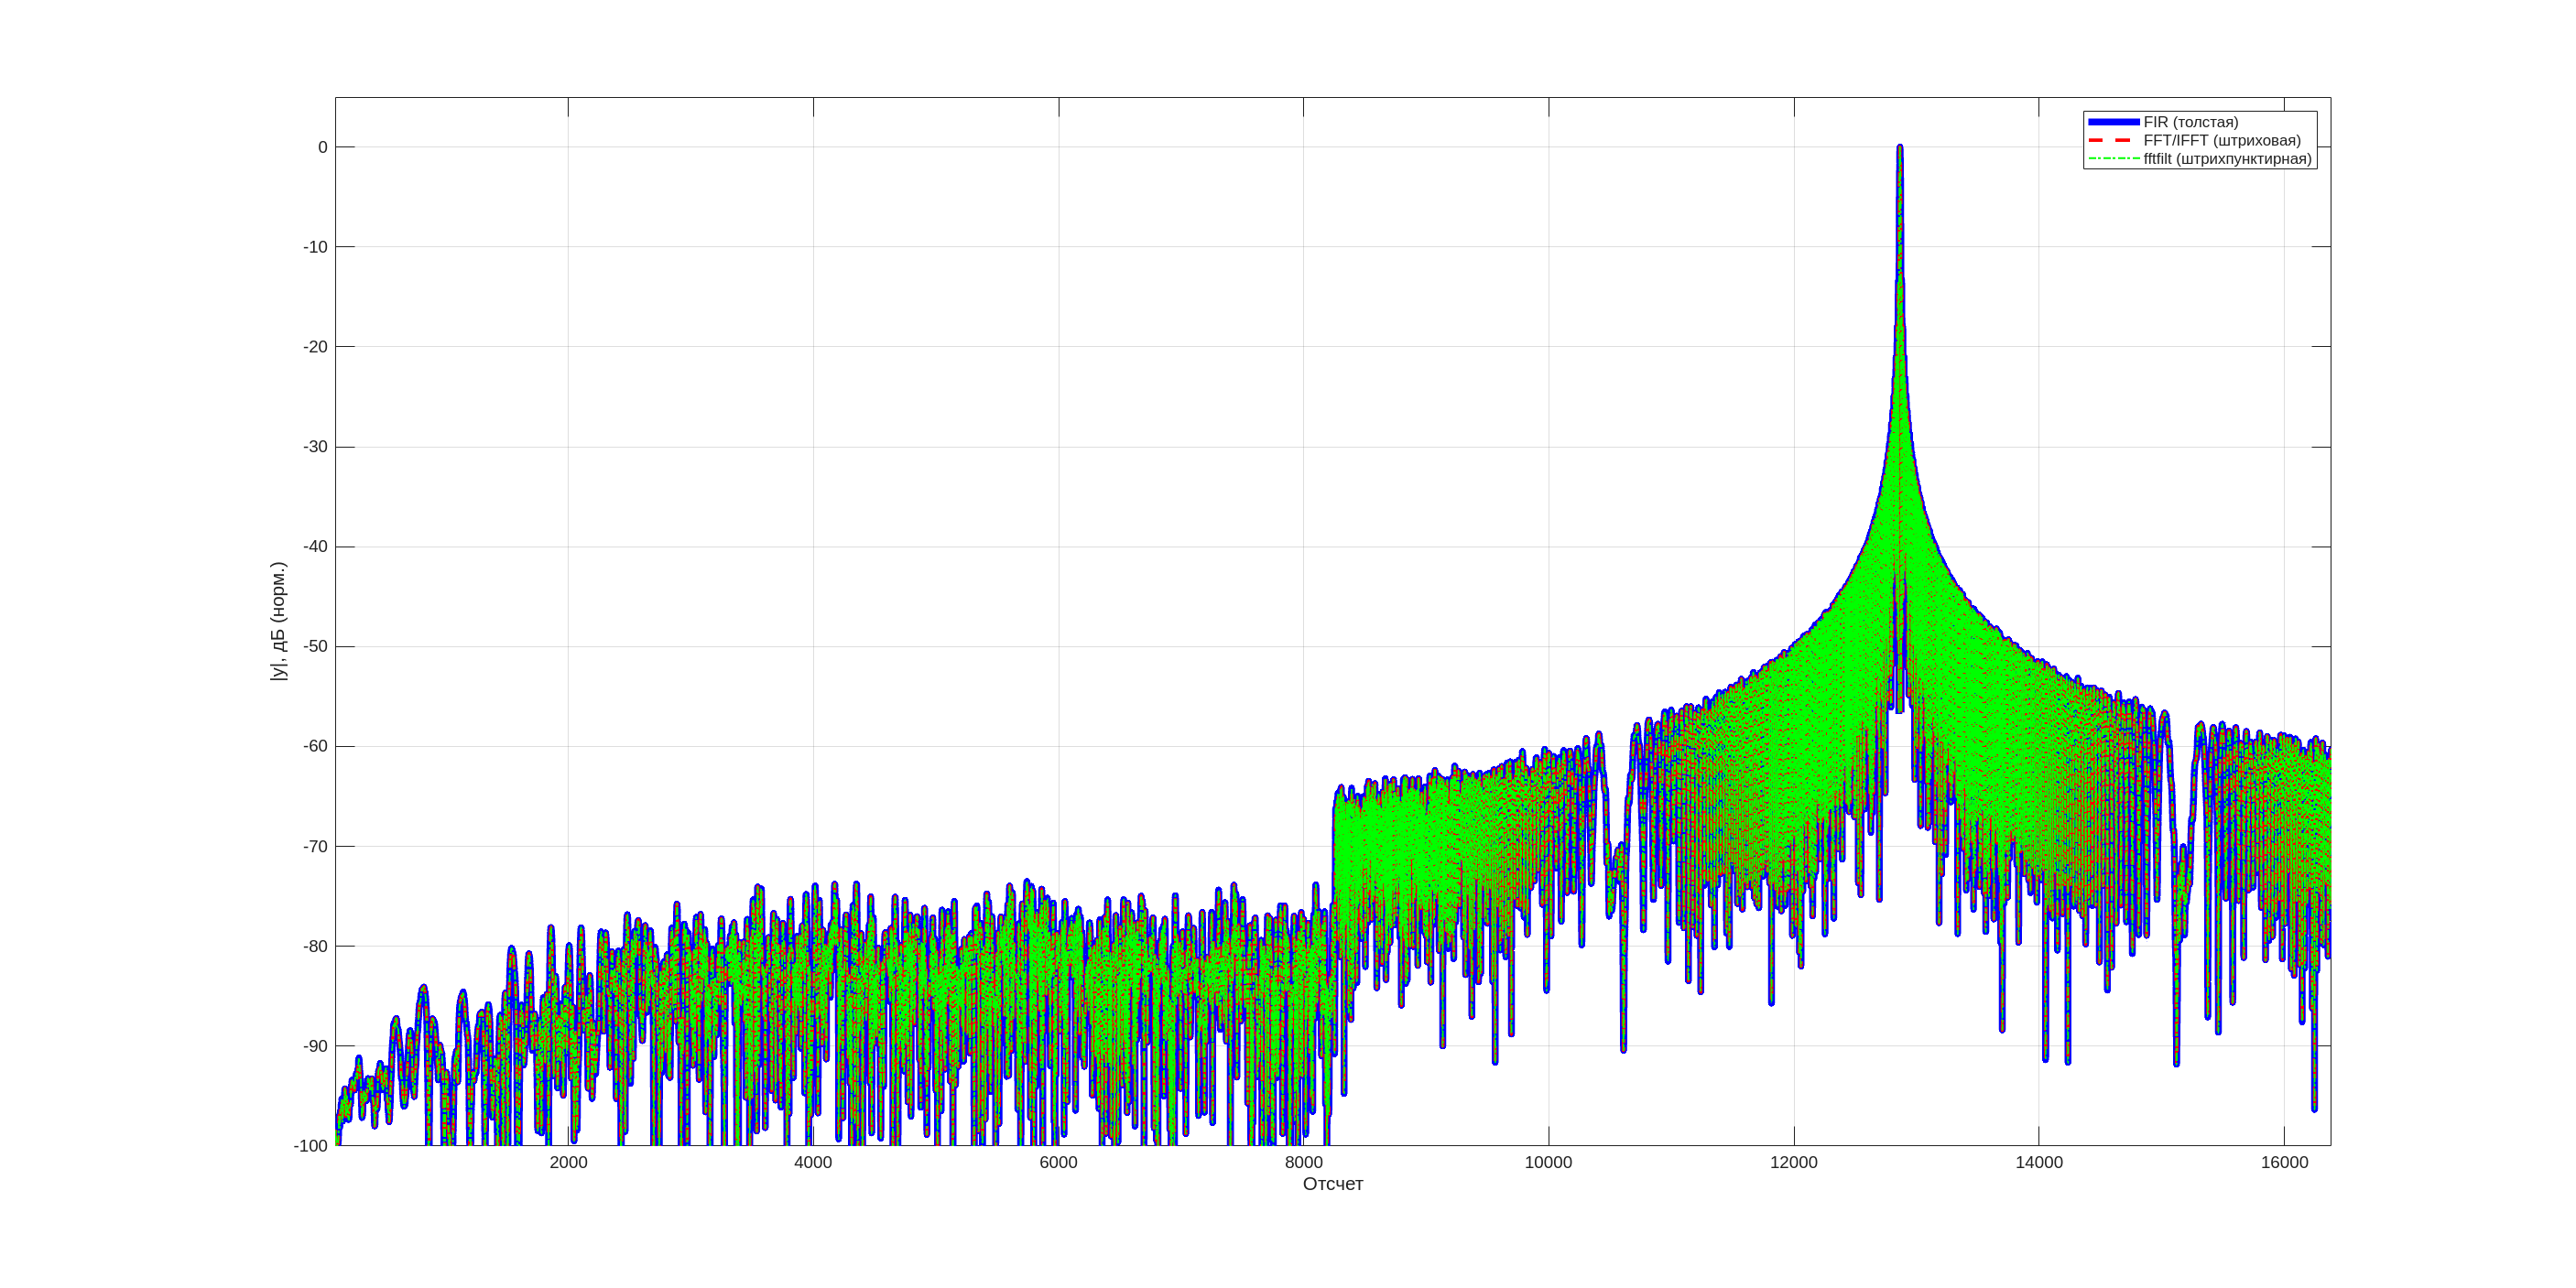
\includegraphics[width=0.85\textwidth]{export_figs/fig_mf_compare.png}
    \caption{Сравнение нормированных характеристик СФ (FIR, FFT/IFFT, fftfilt) во всем периоде зондирования}
    \label{fig:mf_compare}
\end{figure}

Из графика видно, что характеристики всех трех методов полностью совпадают на всех участках временной шкалы, что подтверждает их тождественность. Главный пик сжатого радиоимпульса формируется строго на отсчете $n = 12800$ (сумма задержки $8192$ и длительности $4608$), что соответствует моменту полного накопления энергии сигнала в фильтре. Уровень шума вне зоны сжатия составляет порядка $-75\dots-90$~дБ.

Для детального анализа структуры боковых лепестков и оценки эффекта весовой обработки реплика согласованного фильтра была умножена на окно Хэмминга. На рисунке~\ref{fig:mf_fir} представлен увеличенный фрагмент отклика для метода прямой КИХ-свертки.

\begin{figure}[H]
    \centering
    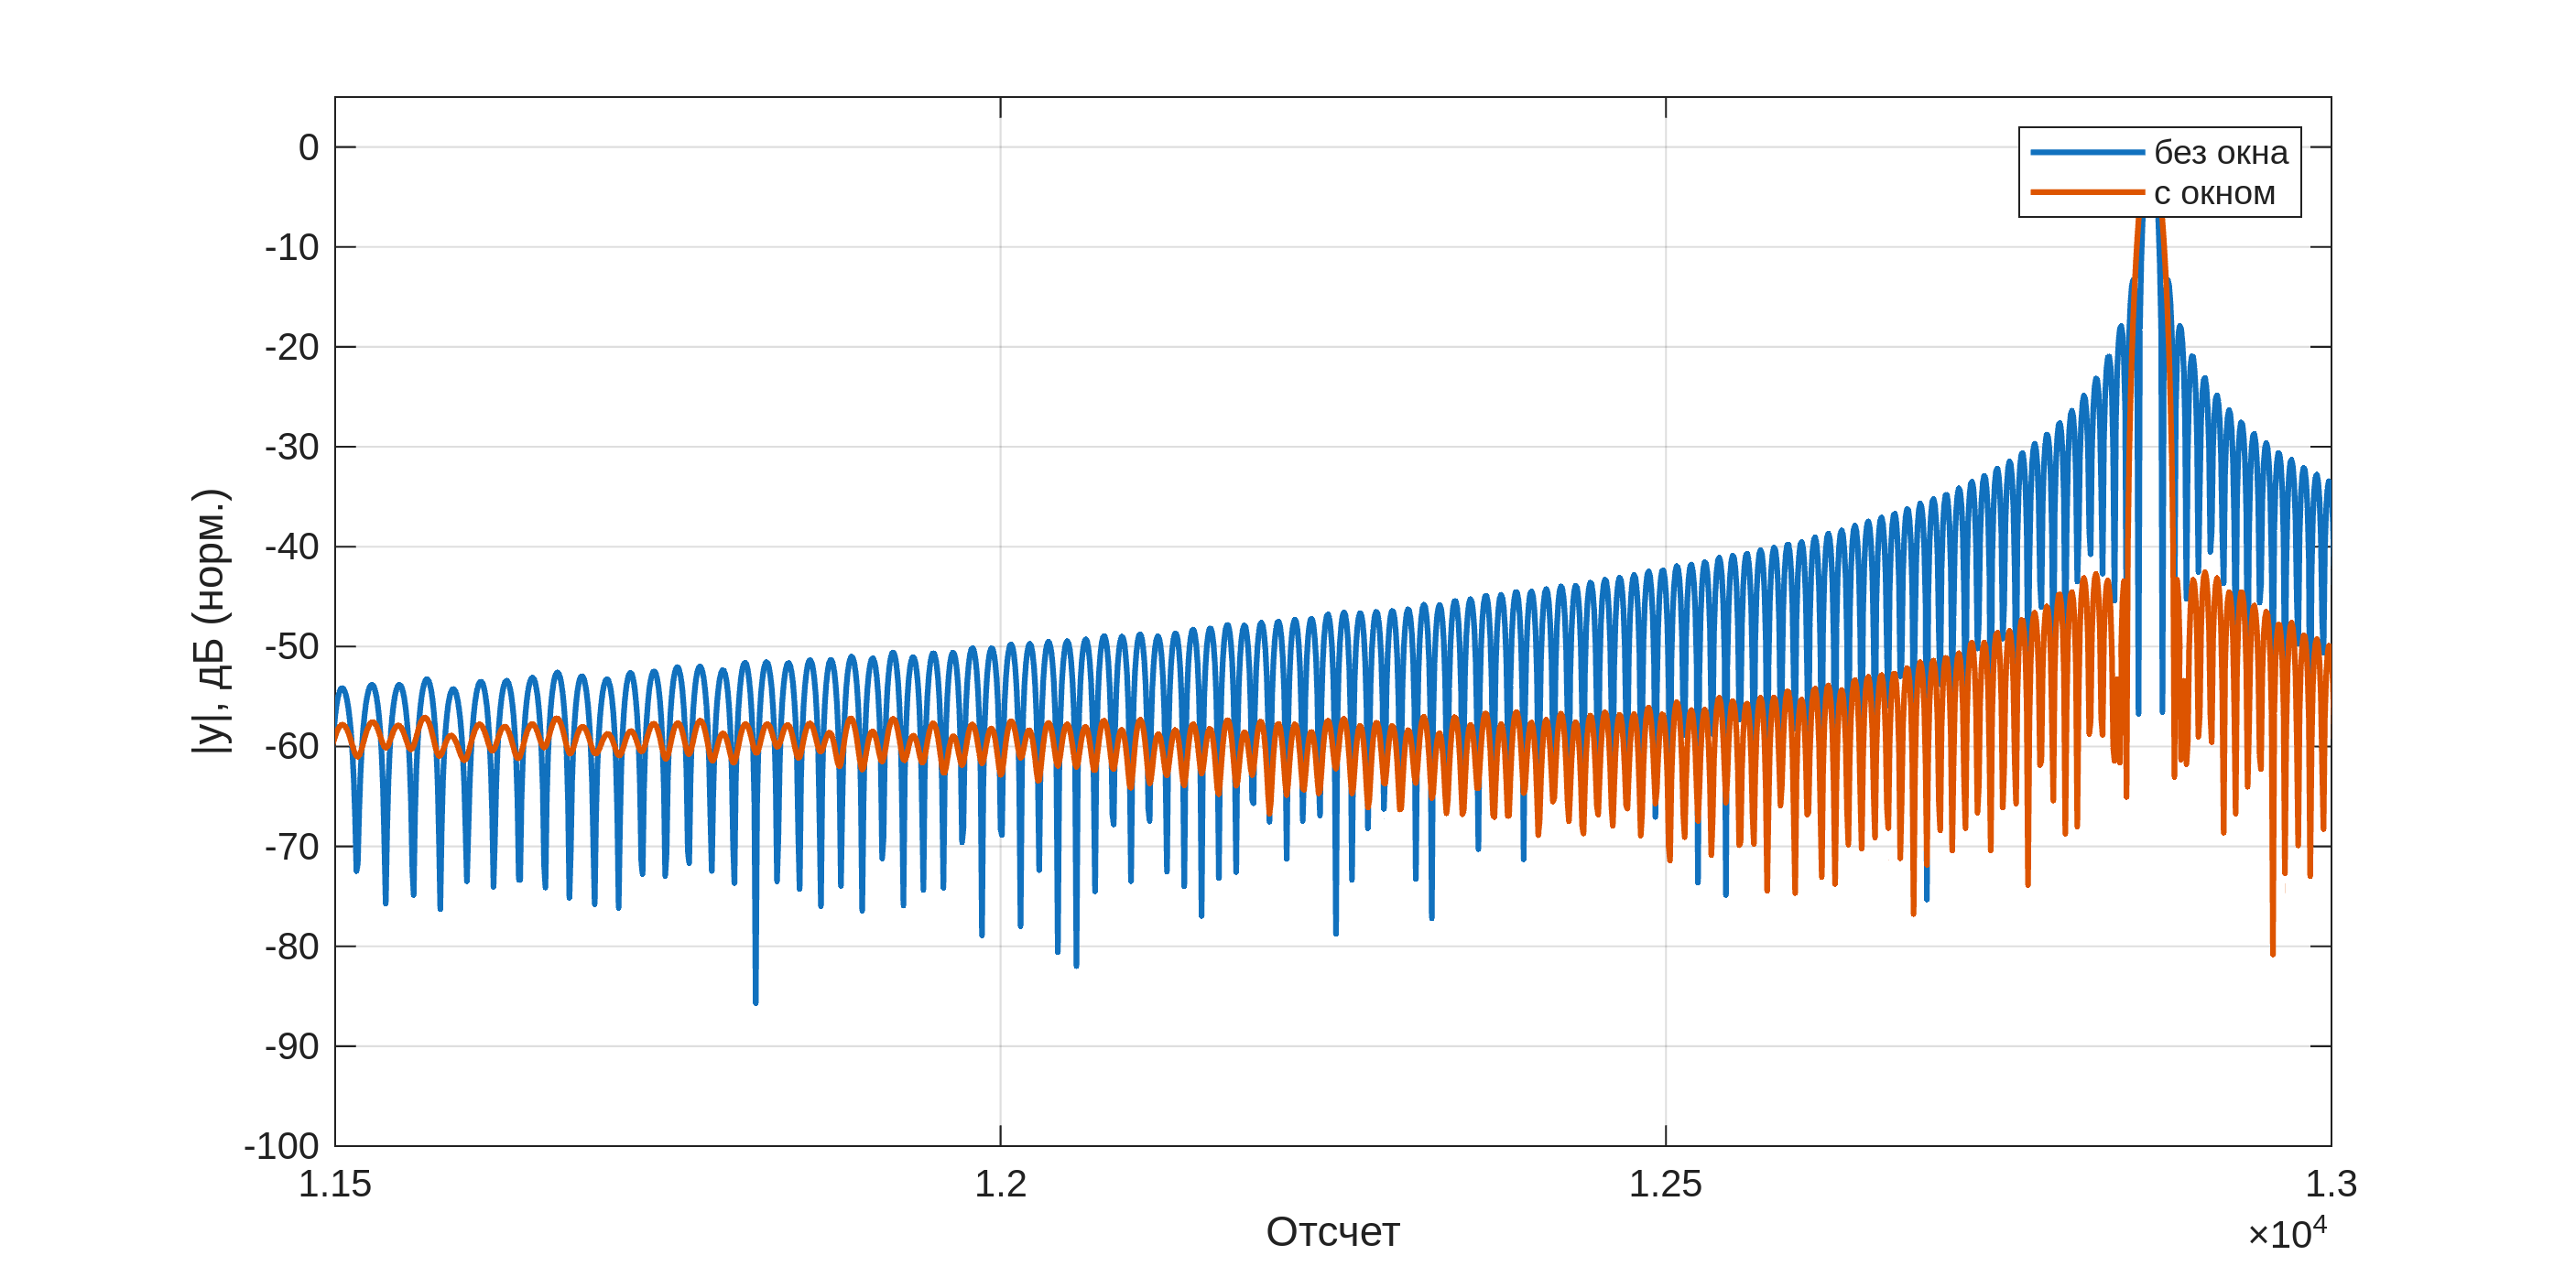
\includegraphics[width=0.85\textwidth]{export_figs/fig_mf_fir.png}
    \caption{Отклик СФ на базе прямой КИХ-свертки: без окна и с окном Хэмминга (зум)}
    \label{fig:mf_fir}
\end{figure}

Без весовой обработки уровень первого бокового лепестка составляет $-13.3$~дБ относительно пика сжатия. Применение окна Хэмминга позволяет снизить уровень ближних боковых лепестков до $-42.8$~дБ, а в дальней зоне подавить их ниже $-55$~дБ ценой уширения центрального пика в $1.35$--$1.4$ раза по уровню $-3$~дБ.

На рисунке~\ref{fig:mf_fft} приведен аналогичный увеличенный фрагмент отклика СФ при расчете спектральным методом через БПФ и ОБПФ.

\begin{figure}[H]
    \centering
    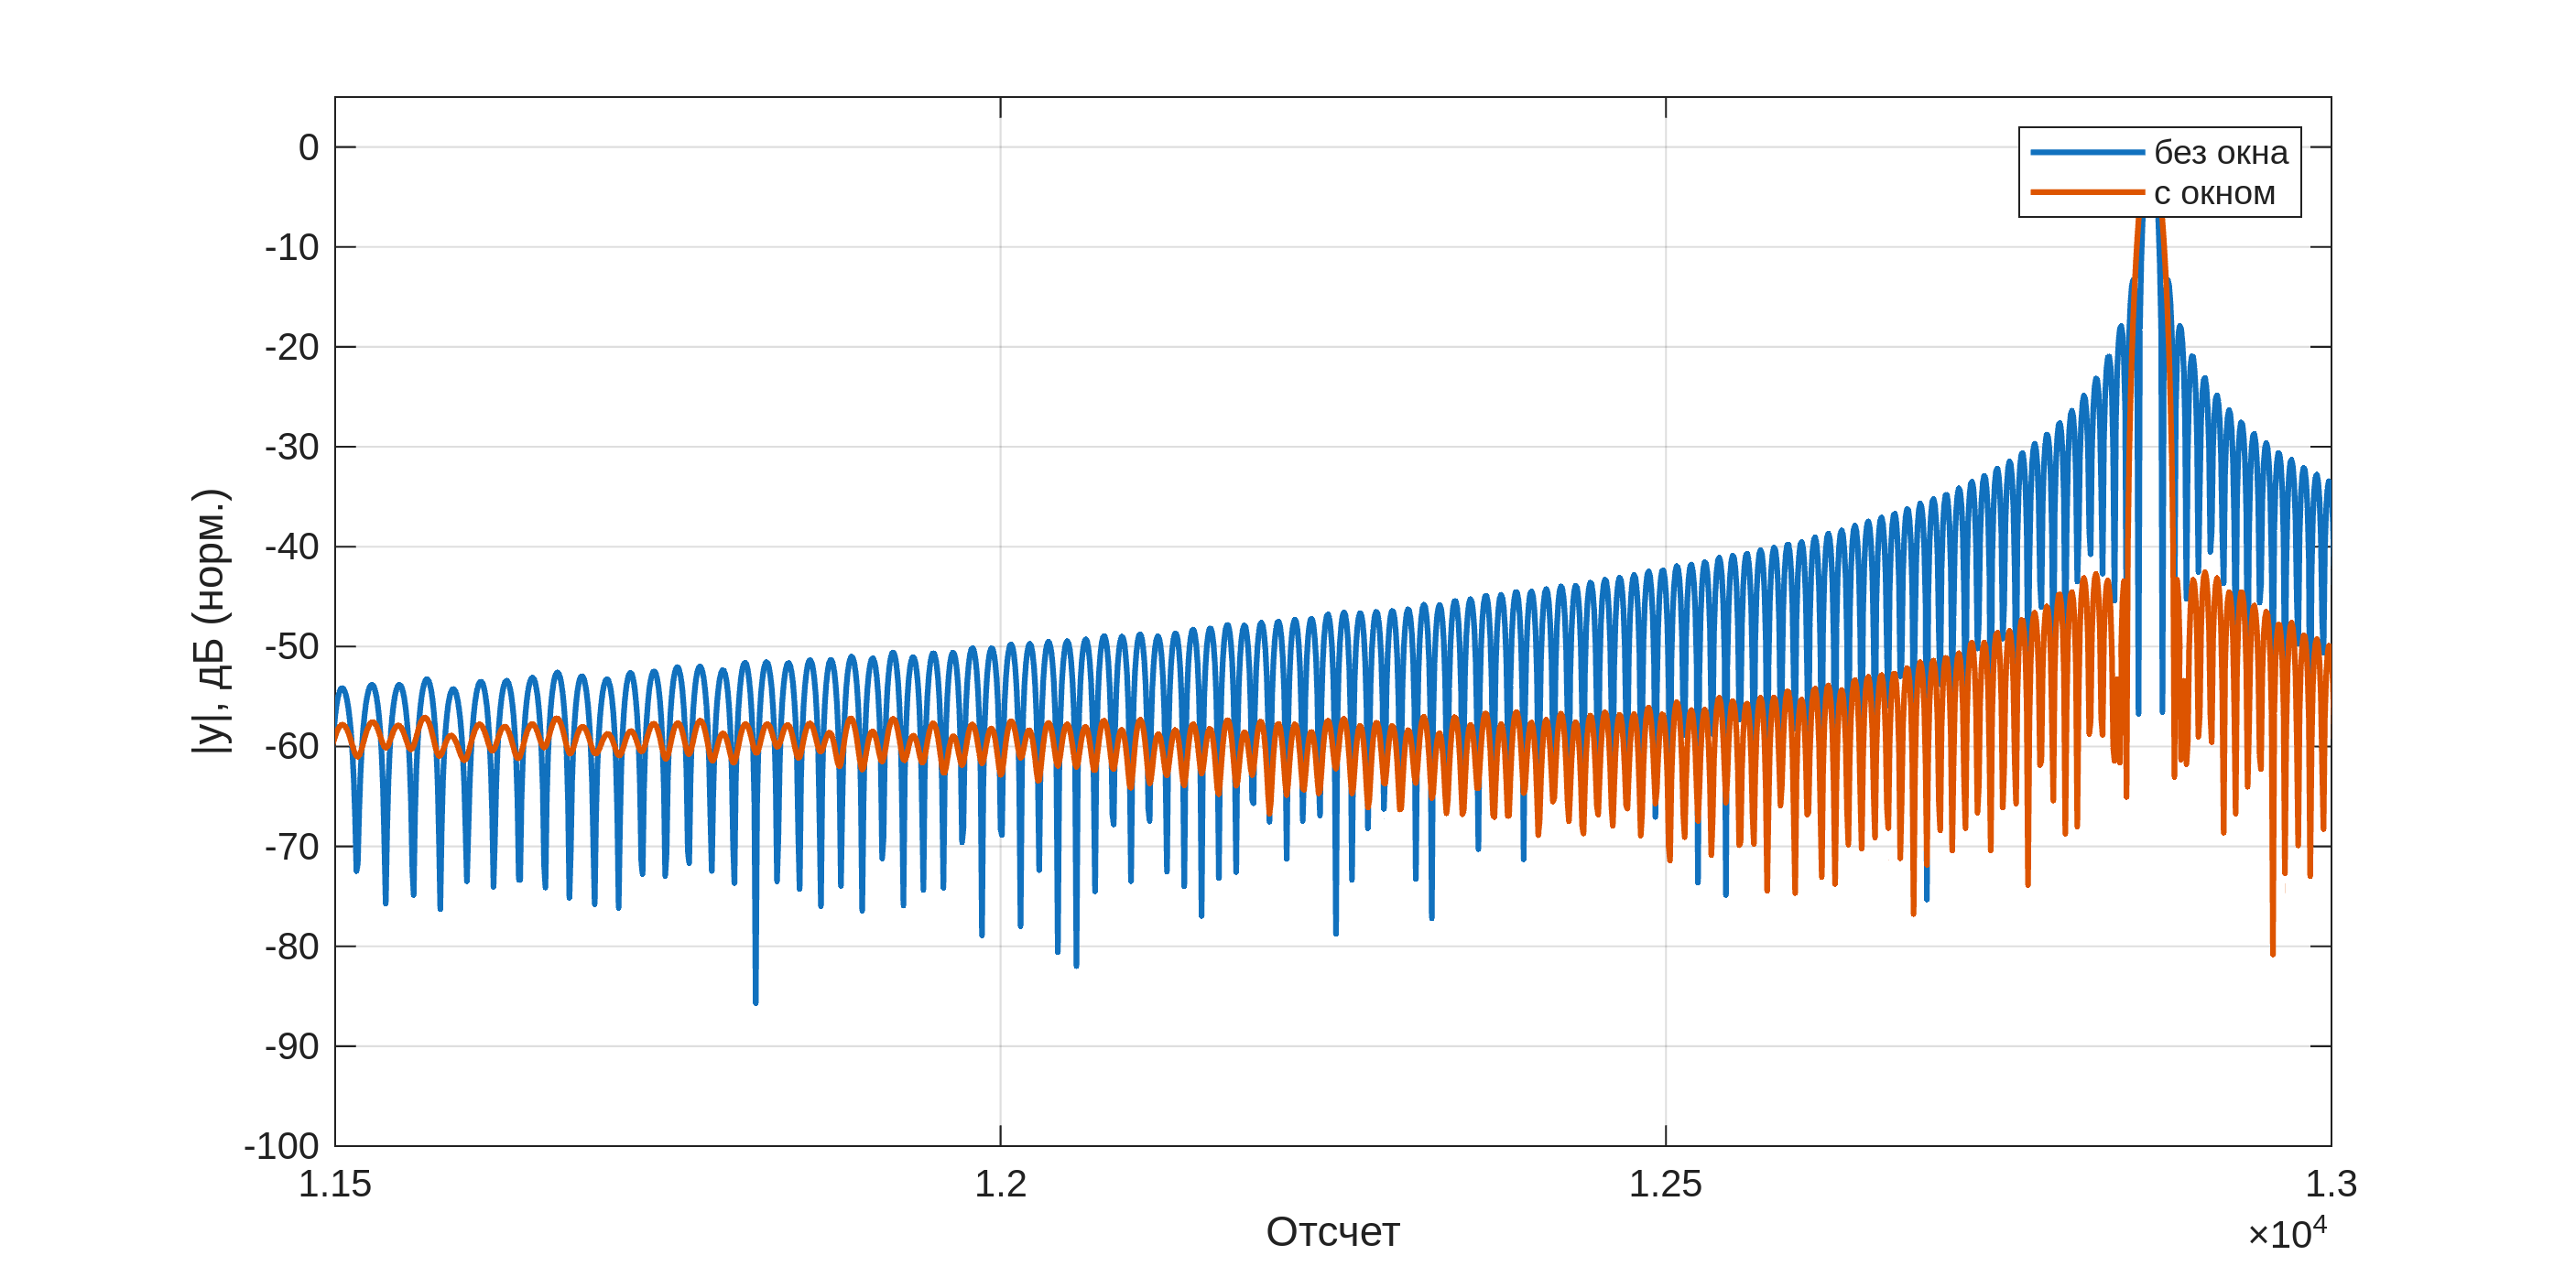
\includegraphics[width=0.85\textwidth]{export_figs/fig_mf_fft.png}
    \caption{Отклик СФ на базе БПФ/ОБПФ: без окна и с окном Хэмминга (зум)}
    \label{fig:mf_fft}
\end{figure}

Спектральный метод демонстрирует полную идентичность с временным подходом: уровень боковых лепестков при взвешивании окном Хэмминга составляет те же $-42.8$~дБ, а пик сжатия сохраняет свою форму и положение во времени.

На рисунке~\ref{fig:mf_fftfilt} показан отклик, полученный методом быстрой блочной свертки \texttt{fftfilt} (Overlap-Add).

\begin{figure}[H]
    \centering
    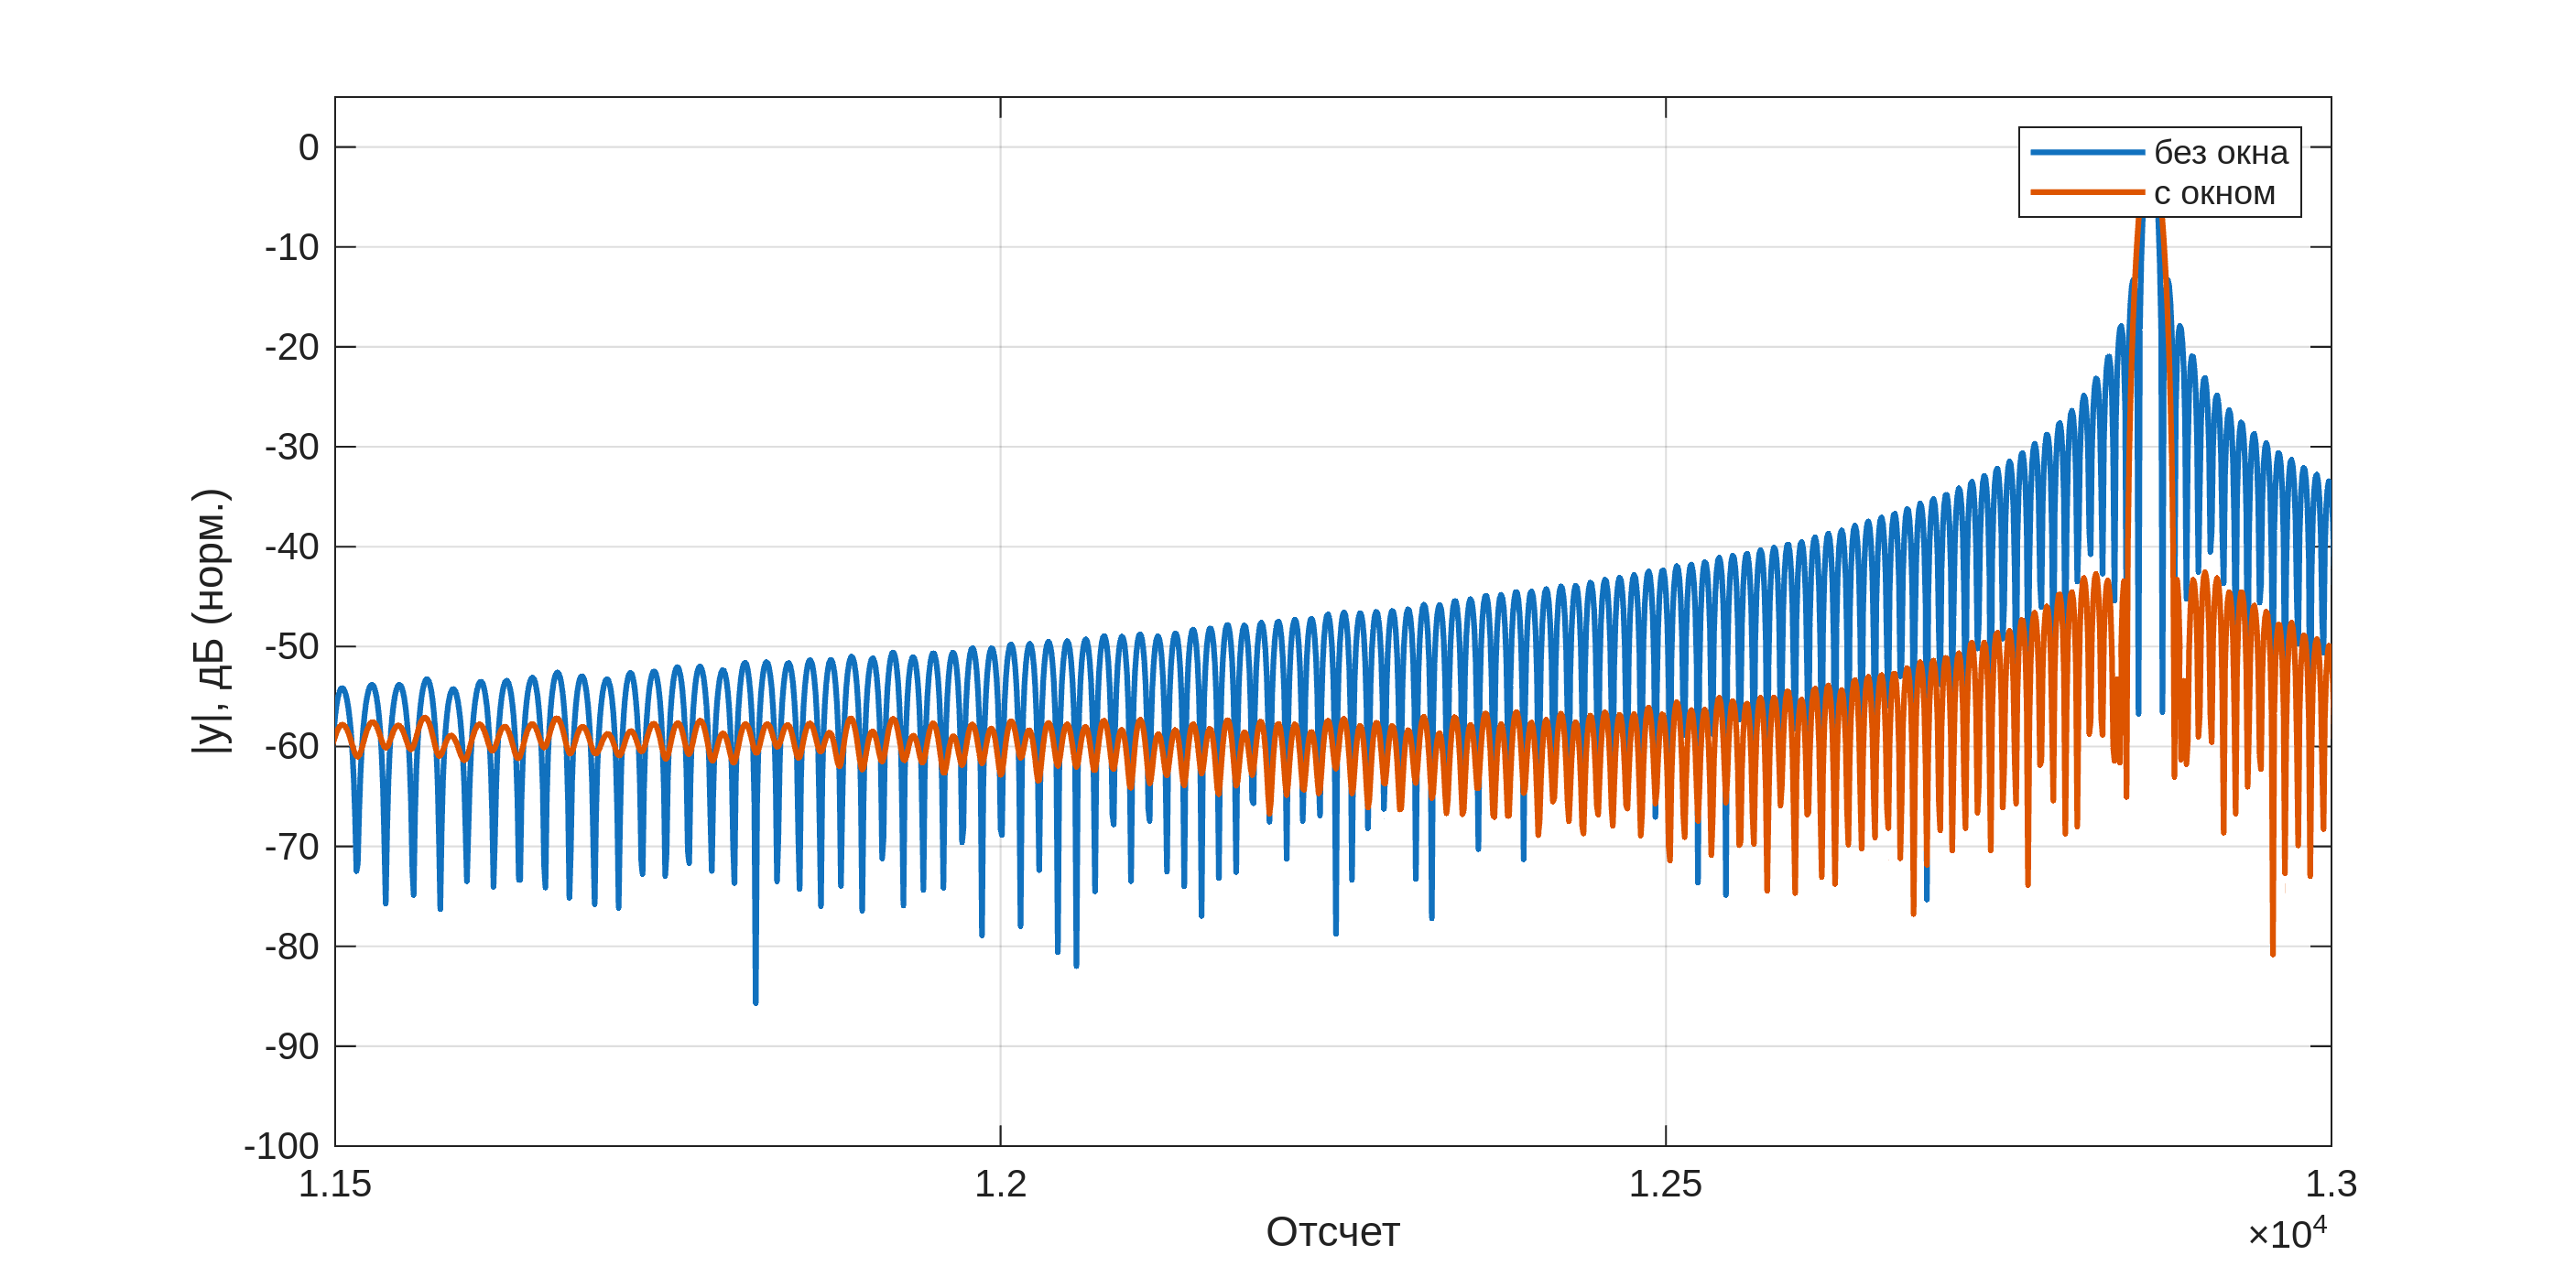
\includegraphics[width=0.85\textwidth]{export_figs/fig_mf_fftfilt.png}
    \caption{Отклик СФ на базе сегментированной быстрой свертки fftfilt (зум)}
    \label{fig:mf_fftfilt}
\end{figure}

Алгоритм \texttt{fftfilt} обеспечивает абсолютно такое же подавление боковых лепестков до уровня $-42.8$~дБ при использовании окна Хэмминга. При этом в отличие от БПФ на всю длину реализации блочный подход позволяет организовать непрерывную конвейерную обработку входных отсчетов в реальном времени без задержки на накопление всего кадра.